The baseline option for the DUNE Cold ADC is a new 16-channel low-noise ADC ASIC intended to read out the LArASIC preamps in the DUNE cold electronics. The ADC is 12 bits and digitizes at a rate of 2 MS/s/channel. The ADC accepts single-ended or differential inputs, and outputs a serial data stream to COLDATA, the DUNE digital serializer chip. The ADC ASIC is implemented using 65 nm CMOS technology. The ASIC uses a conservative, industry standard design along with digital calibration. A block diagram of the ADC ASIC is shown in Figure~\ref{fig:adc-blockdiagram}. The design and testing of the baseline ADC ASIC is being carried out by a collaboration of scientists and engineers at BNL, Fermilab, and LBNL.

\begin{dunefigure}
[Baseline cold ADC ASIC block diagram.]
{fig:adc-blockdiagram}
{Baseline cold ADC ASIC block diagram.}
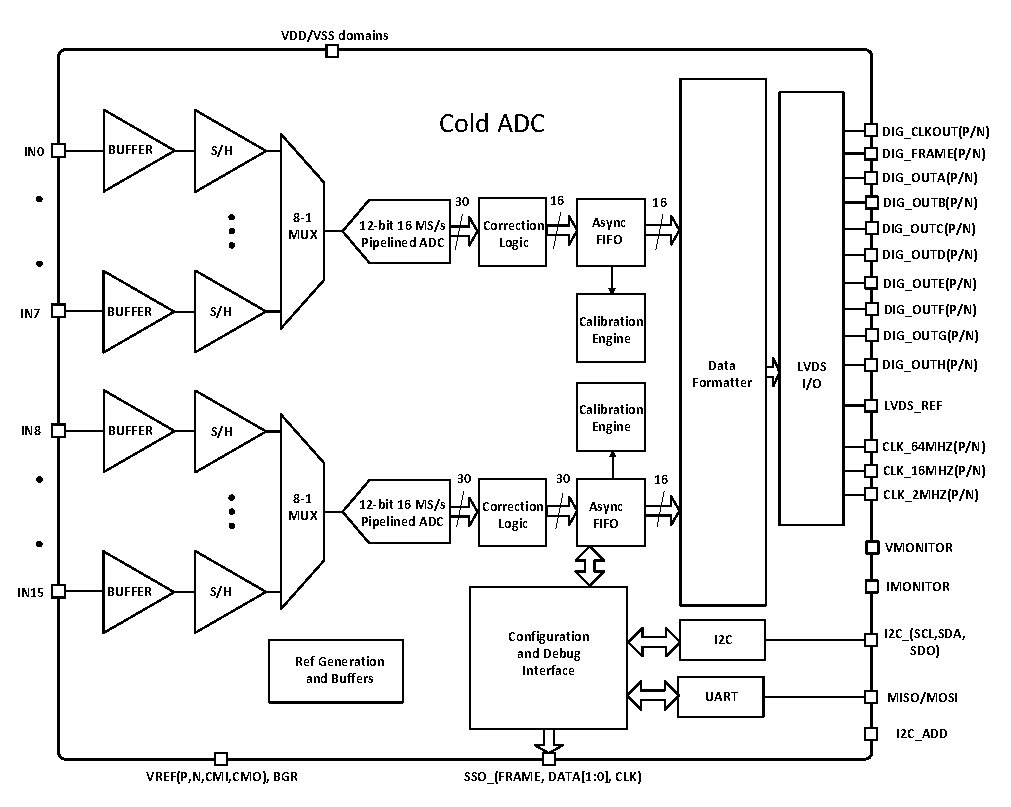
\includegraphics[width=0.75\textwidth]{tpcelec-ADCChipBlockDiagram.pdf}
\end{dunefigure}

Each Cold ADC receives 16 single-ended voltage outputs from a single LArASIC chip. The voltage is buffered and then sampled at a rate of 2 MS/s. The analog samples are multiplexed by 8 and digitized by calibrated 12-bit pipelined ADCs operating at 16 MS/s. The ADC uses the well-known Pipelined architecture with redundancy to reduce the impact of component non-idealities on the linearity of the ADC~\cite{121557}. The linearity of the raw output samples from the ADCs is improved using an on-chip calibration. The corrected ADC output is then multiplexed onto eight LVDS channels and sent to COLDATA for further aggregation and transmission via a copper link to the warm electronics sitting outside the cryostat.

The ADC ASIC is designed for low-noise operation. The noise specification is 175~\si{\micro}V RMS. This noise specification was chosen to ensure that LArASIC will dominate the overall noise performance of the channel.

The ADC is digitally calibrated using the proven Soenen-Karanicolas algorithm~\cite{280084,372864}. The algorithm exploits the observation that in a pipelined ADC with redundancy, the ADC nonlinearity is caused almost entirely by errors in the closed-loop interstage gain~\cite{121557}. Traditionally, the ADC output bits are assumed to be in radix 2 and are simply combined to generate the ADC output. However, due to unavoidable non-idealities such as finite op-amp gain and capacitor mismatch, the true radix of each stage is slightly different from two. The extent to which the true radix is different from two leads to DNL and INL in the ADC transfer characteristic. The Soenen-Karanicolas algorithm provides a way to measure the radix of a given stage by forcing events at the decision boundaries and using the following stages of the ADC to record the stage's response. The radix is then decomposed into a set of weights and during normal operation the ADC output is converted from the true radix to radix 2 using pipelined digital adders. This way, static linearity can be greatly improved without any post-processing required. To provide additional ease-of-use, all calibration hardware (including test signal generation) is included on the ADC ASIC. To control power dissipation, the stages of the ADC are scaled in area to take advantage of the fact that the accuracy requirements of the stages decline down the pipeline~\cite{494191}.

To reduce the number of pads and to improve performance all required reference voltages and currents are generated internally by a resistor-programmed reference generator on the ASIC.

The Cold ADC is highly configurable (see Table~\ref{tab:ADCconfig}) and includes two redundant slow control interfaces for configuration (either UART or I2C). The configurability of the chip is included primarily to reduce risk by providing a high degree of flexibility and observability. First, many of the components on the ASIC can be bypassed and their functions assumed at the board level if desired. For example, the ADC reference voltages can be supplied externally and the input buffers can be bypassed. Second, the ADC digital calibration algorithm can be implemented externally with the calculated stage weights loaded back into the chip using the configuration interface. Third, various internal voltages and currents can be monitored and test data can be introduced at various parts of the digital processing to observe the function of the ASIC. Lastly, the bias point of the analog circuits in the ASIC can be adjusted to compensate for expected component variations between room temperature and liquid Argon temperature.

\begin{dunetable}
[Baseline cold ADC ASIC configurability.]
{p{3cm} p{9cm} p{4cm}}
{tab:ADCconfig}
{Baseline cold ADC ASIC configurability.}
\textbf{BLOCK} &\textbf{Configurability} & \textbf{Comment}\\ \toprowrule
Input Buffer & Single-ended/differential, bypass, bias current adjust & Reduces design risk \\ \colhline
Sample-and-hold Amplifiers & Multiplexer freeze, bias current adjust & Simplifies evaluation of prototype \\ \colhline
ADC & Bias currents, clock edge fine adjustment, sync and test modes & Simplifies evaluation of prototype and reduces risk \\ \colhline
References & All reference voltages can be adjusted in 8~mV increments; all references can be powered down and external voltages used & Reduces design risk \\ \colhline
Calibration & Number of stages and amount of digital filtering; all calibration commands can be implemented through configuration interface for offline calibration; known data can be injected at various points for testing & Simplifies evaluation of prototype and reduces risk \\ \colhline
Output Monitor & Various internal bias voltages and currents can be sent off-chip for evaluation & Simplifies evaluation of prototype \\
\end{dunetable}

%References:
%[1] S.H. Lewis, H.S. Fetterman, G.F. Gross, R. Ramachandran, and T.R. Viswanathan, “A 10-b 20-Msample/s analog-to-digital converter,” IEEE J. Solid-State Circuits, vol. 27, no. 3, pp. 351–358, March 1992.
%[2] A.N Karanicolas, H.S. Lee, and K.L. Bacrania, “A 15-b 1-Msample/s digitally self-calibrated ADC,” IEEE J. Solid-State Circuits, vol. 28, no. 12, pp. 1207–1215, December 1993.
%[3] E.G. Soenen and R.L. Geiger, “An architecture and an algorithm for fully digital correction of monolithic pipelined ADCs,” IEEE Trans. Circuits Syst. II, vol. 42, no. 3, pp. 143–153, March 1995.
%[4] D.W Cline and P.R. Gray, “A power optimized 13-b 5 Msamples/s pipelined analog-to-digital Converter in 1.2 µm CMOS,” IEEE J. Solid-State Circuits, vol. 31, no. 3, pp. 294–303, March 1996.
